\documentclass[twoside]{article}
\usepackage[french]{babel}
\usepackage[T1]{fontenc}
\usepackage[left=2cm,right=2cm,top=2cm,bottom=2cm]{geometry}
\usepackage{fancyhdr}
\pagestyle{fancy}
\fancyfoot[LE]{\thepage}
\fancyfoot[RO]{\thepage}
\fancyfoot[C]{}
%\usepackage{anyfontsize}

\usepackage{fontspec}
\defaultfontfeatures{Ligatures=TeX}
%\setmainfont[Mapping=tex-text]{Sitka Display}
\usepackage[small,sf,bf]{titlesec}

\usepackage{graphicx}
\usepackage{xcolor, colortbl}
\usepackage{sectsty}

\definecolor{DarkGreen}{HTML}{384d3e}
\definecolor{PureWhite}{HTML}{FFFFFF}
\definecolor{DarkRed}{HTML}{6e272d}
\definecolor{DarkGold}{HTML}{a48e3b}

\sectionfont{\color{DarkGreen}}
\subsectionfont{\color{DarkRed}}
\subsubsectionfont{\color{DarkGold}}

\begin{document}

\title{\vspace{8cm}{\Huge Star Wars aux confins de l'empire} \\ \vspace{2cm} 
\includegraphics{../img/logo}}

\date{}



\maketitle
\vspace{4cm}
Ce document n’a pas pour rôle d'expliquer tous les détails (le livre de règles est là pour ça !) quant à la création de voter personnage, mais de vous résumer les choix et les options pendant la création. Bien sûr, tout choix doit se faire avec l’approbation du MJ.
\clearpage
\tableofcontents
\clearpage

\section{Déterminer le concept et l'historique du personnage (ldr p. 36)}

C'est le moment de vous faire une idée de ce que vous voulez comme personnage, qu'a-t-il fait par le passé, quels sont ses buts? Pour plus détails reportez-vous à la page 36 de votre livre de règles.

\section{Déterminer l'obligation de départ (ldr p. 38)}
Vous devez choisir une Obligation départ soit la sélectionner par les dés. L'Obligation représente la pression mise sur votre personnage, ajoutant du piquant à l'aventure :

\renewcommand{\arraystretch}{1.4}
\begin{center}
	\begin{tabular}{|p{4.5cm}|p{12cm}|}
		\hline 
		\cellcolor{DarkRed} {\large \textcolor{PureWhite}{\textbf{D100}}} & \cellcolor{DarkRed} {\large \textcolor{PureWhite}{\textbf{Type d'obligation}}} \\
		\hline 
		01 -- 08 & \textbf{Addiction} : vous êtes soumis à une addiction (au choix du joueur sous couvert du MJ). Moins le personnage assouvit son addiction, plus celui-ci a du mal à se concentrer sur les tâches banales, ce qui se traduit le plus souvent par l'ajout de {\Large 
\includegraphics[height=\fontcharht\font`\B]{../img/dice_black}} à {\Large 
\includegraphics[height=\fontcharht\font`\B]{../img/dice_black}} {\Large 
\includegraphics[height=\fontcharht\font`\B]{../img/dice_black}} {\Large 
\includegraphics[height=\fontcharht\font`\B]{../img/dice_black}} aux tests de compétence. \\
		\hline 
		09 -- 16 & \textbf{Trahison} : soit le personnage est victime d'une trahison soit c'est le traitre lui-même. \\
		\hline 
		17 -- 24 & \textbf{Chantage} : quelqu'un a découvert un de pires secrets du personnage. \\
		\hline 
		25 -- 32 & \textbf{Prime} : pour une raison ou pour une autre la tête du personnage est mise à prix. \\
		\hline 
		33 -- 40 & \textbf{Criminel} : le personnage à un passé criminel, ou a été accusé a tort d'un crime. \\
		\hline 
		41 -- 48 & \textbf{Dette} : le personnage doit quelque chose à quelqu'un. \\
		\hline 
		49 -- 56 & \textbf{Obligé} : le personnage est animé par un profond sens du devoir. A la différence du serment, le PJ entretien un lien légal ou rituel avec une organisation qui lui rend la vie impossible quand il se dérobe à ses engagements. \\
		\hline 
		57 -- 64 & \textbf{Famille} : le personnage entretient des liens étroits avec sa famille, ce qui nécessite beaucoup de temps et d'attention. \\
		\hline 
		65 -- 72 & \textbf{Faveur} : le personnage doit une grosse faveur, quoiqu'il en soit on lui demandera surement de rendre la pareille. \\
		\hline 
		73 -- 80 & \textbf{Serment} : le personnage a fait une promesse qui dicte ses pensées et actions. \\
		\hline 
		81 -- 88 & \textbf{Obsession} : le personnage à une obsession malsaine qui l'incommode au quotidien. \\
		\hline 
		89 -- 96 & \textbf{Responsabilité} : le personnage se sent particulièrement responsable d'une personne, d'un lieu ou d'une chose. \\
		\hline 
		97 -- 00 & Tirez deux fois sur la table, L'obligation de départ est divisée en deux origines (le poids est aussi divisé en deux pour chaque Obligation) \\
		\hline 
	\end{tabular}
\end{center}

Il est possible, pour avoir un bonus d'xp ou de crédits, d'alourdir son Obligation de départ comme dans ce tableau (p. 40) :
\begin{center}
	\begin{tabular}{|p{4.5cm}|p{4cm}|}
		\hline 
		\cellcolor{DarkRed} {\large \textcolor{PureWhite}{\textbf{Bonus}}} & \cellcolor{DarkRed} {\large \textcolor{PureWhite}{\textbf{Coût}}} \\
		\hline 
		+ 5 XP de départ & Obligation + 5 \\
		\hline 
		+ 10 XP de départ & Obligation +10 \\
		\hline
		+ 1.000 crédits de départ & Obligation + 5 \\
		\hline
		+ 2.500 crédits de départ & Obligation +10 \\
		\hline
	\end{tabular}
\end{center}

\section{Choisir l'espèce du personnage (ldr p. 43)}
La galaxie foisonne d'espèces douées de conscience qui ont toutes leur lot de capacités et de croyances. Le joueur doit choisir son espèce. Une fois cette décision prise, impossible de revenir sur ce choix :

\subsection*{Bothans}

\noindent\begin{minipage}{0.3\textwidth}
	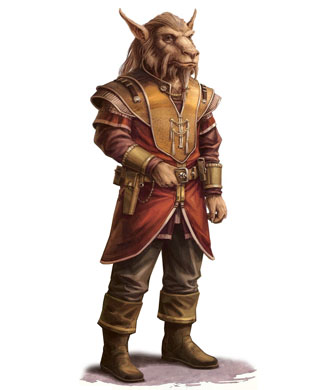
\includegraphics[width=1\linewidth]{../img/species/bothan}
\end{minipage}%
\hfill%
\begin{minipage}{0.7\textwidth}\raggedleft
	\begin{itemize}
		\item \textbf{Seuil de blessure :} 10 + Vigueur 
		\item \textbf{Seuil de stress :} 11 + Volonté 
		\item \textbf{Expérience de départ :} 100 XP
		\item \textbf{Capacité spéciale :} les Bothans commencent le jeu avec 1 rang en \textbf{Système D}. Ils ne peuvent cependant pas dépasser le rang 2 dans cette compétence à la création de perso. Ils commencent également avec 1 rang de \textbf{Persuasion}.
	\end{itemize}
\end{minipage}

\subsection*{Droïdes}

\noindent\begin{minipage}{0.3\textwidth}
	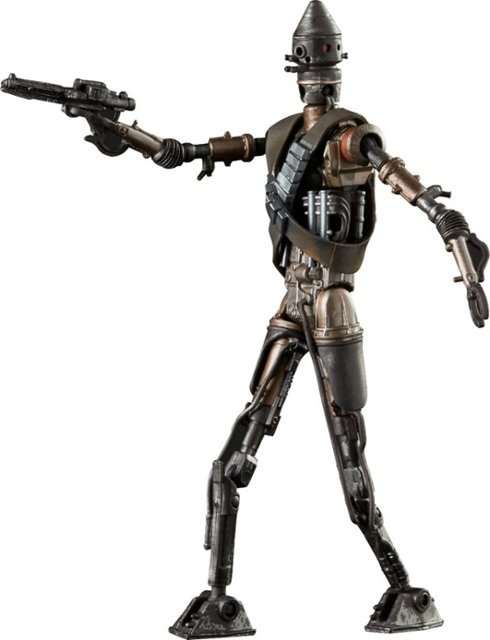
\includegraphics[width=1\linewidth]{../img/species/droid}
\end{minipage}%
\hfill%
\begin{minipage}{0.7\textwidth}\raggedleft
	\begin{itemize}
		\item \textbf{Seuil de blessure :} 10 + Vigueur 
		\item \textbf{Seuil de stress :} 10 + Volonté 
		\item \textbf{Expérience de départ :} 175 XP
		\item \textbf{Capacité spéciale :} les Droïdes ne mangent pas, ne dorment pas, ne respirent pas. La limitation d'implant est de 6. Une fois sa carrière choisie il gagne un rang dans 6 des 8 compétences de carrière (au lieu de 4), une fois sa spécialité choisie il gagne un rang dans 3 des 4 compétences de spécialités (au lieu de 2). \textbf{Inorganique :} les Droïdes étant inorganiques, les cuves bacta, stimpacks et tests de médecine sont inopérants. Ils récupèrent en se reposant. Autrement on peut s'en occuper avec des tests de mécaniques, les trousses de mécaniques s'utilisent comme les stimpacks. Pour plus de détails voir page 220. \textbf{Être mécanique : }les Droïdes ne peuvent pas être affectés par les pouvoirs de la Force qui influencent l'esprit, et ne peuvent non plus avoir de valeur de Force.
	\end{itemize}
\end{minipage}

\subsection*{Humains}

\noindent\begin{minipage}{0.3\textwidth}
	
\includegraphics[width=1\linewidth]{../img/species/human}
\end{minipage}%
\hfill%
\begin{minipage}{0.7\textwidth}\raggedleft
	\begin{itemize}
		\item \textbf{Seuil de blessure :} 10 + Vigueur 
		\item \textbf{Seuil de stress :} 10 + Volonté 
		\item \textbf{Expérience de départ :} 110 XP
		\item \textbf{Capacité spéciale :} les Humains commencent le jeu avec 1 rang dans 2 compétences hors carrière de leur choix. Ils ne peuvent cependant pas dépasser le rang 2 dans ces compétences à la création de perso.
	\end{itemize}
\end{minipage}

\subsection*{Gands}

\noindent\begin{minipage}{0.3\textwidth}
	
\includegraphics[width=1\linewidth]{../img/species/gand}
\end{minipage}%
\hfill%
\begin{minipage}{0.7\textwidth}\raggedleft
	\begin{itemize}
		\item \textbf{Seuil de blessure :} 10 + Vigueur 
		\item \textbf{Seuil de stress :} 10 + Volonté 
		\item \textbf{Expérience de départ :} 100 XP
		\item \textbf{Capacité spéciale :} les Gands commencent le jeu avec 1 rang en \textbf{Sang Froid}. Ils ne peuvent cependant pas dépasser le rang 2 dans cette compétence à la création de perso.\textbf{		Respirateurs d'ammoniac :} Soit le Gand a des poumons et donc un respirateur d'ammoniac, il traite l'oxygène comme une atmosphère dangereuse de niveau 8 et gagne +10 xp de départ, soit il n'en a pas et trouve son ammoniac dans sa nourriture, et est immunisé contre la suffocation (mais pas contre les blessures que l'on subit dans le vide).
	\end{itemize}
\end{minipage}

\subsection*{Rodiens}

\noindent\begin{minipage}{0.3\textwidth}
	
\includegraphics[width=1\linewidth]{../img/species/rodien}
\end{minipage}%
\hfill%
\begin{minipage}{0.7\textwidth}\raggedleft
	\begin{itemize}
		\item \textbf{Seuil de blessure :} 10 + Vigueur 
		\item \textbf{Seuil de stress :} 10 + Volonté 
		\item \textbf{Expérience de départ :} 100 XP
		\item \textbf{Capacité spéciale :} les Rodiens commencent le jeu avec 1 rang en \textbf{Survie}. Ils ne peuvent cependant pas dépasser le rang 2 dans cette compétence à la création de perso. Les Rodiens commencent aussi avec 1 rang dans le talent \textbf{Pisteur chevronné}.
	\end{itemize}
\end{minipage}

\subsection*{Trandosiens}

\noindent\begin{minipage}{0.3\textwidth}
	
\includegraphics[width=1\linewidth]{../img/species/trandoshan}
\end{minipage}%
\hfill%
\begin{minipage}{0.7\textwidth}\raggedleft
	\begin{itemize}
		\item \textbf{Seuil de blessure :} 12 + Vigueur 
		\item \textbf{Seuil de stress :} 9 + Volonté 
		\item \textbf{Expérience de départ :} 90 XP
		\item \textbf{Capacité spéciale :} les Trandosiens commencent le jeu avec 1 rang en \textbf{Perception}. Ils ne peuvent cependant pas dépasser le rang 2 dans cette compétence à la création de perso. \textbf{Régénération :} quand un Trandosien se débarrasse d'une blessure en se reposant ou dans une cuve bacta, il en élimine une de plus. Cela ne fonctionne pas avec des premiers soins, stimpacks ou tests de médecine. Les membres aussi peuvent se régénérer, mais il faut au moins attendre un mois pour qu'ils soient utilisables. \textbf{Griffe :} quand un Trandosien effectue des tests de \textbf{Pugilat} pour infliger des dégâts, il inflige +1 dégât et a une valeur de critique de 3.
	\end{itemize}
\end{minipage}

\subsection*{Twi'leks}

\noindent\begin{minipage}{0.3\textwidth}
	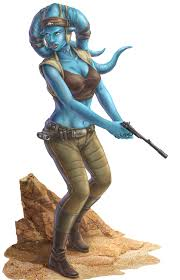
\includegraphics[width=1\linewidth]{../img/species/twilek}
\end{minipage}%
\hfill%
\begin{minipage}{0.7\textwidth}\raggedleft
	\begin{itemize}
		\item \textbf{Seuil de blessure :} 10 + Vigueur 
		\item \textbf{Seuil de stress :} 11 + Volonté 
		\item \textbf{Expérience de départ :} 100 XP
		\item \textbf{Capacité spéciale :} les Tw'ileks commencent le jeu avec 1 rang en \textbf{Charme} ou en \textbf{Tromperie}. Ils ne peuvent cependant pas dépasser le rang 2 dans la compétence choisie à la création de perso. Quand ils effectuent un test de compétence, ils peuvent retirer {\Large 
\includegraphics[height=\fontcharht\font`\B]{../img/dice_black}} dû à des conditions environnementales chaudes ou arides.
	\end{itemize}
\end{minipage}

\subsection*{Wookies}

\noindent\begin{minipage}{0.3\textwidth}
	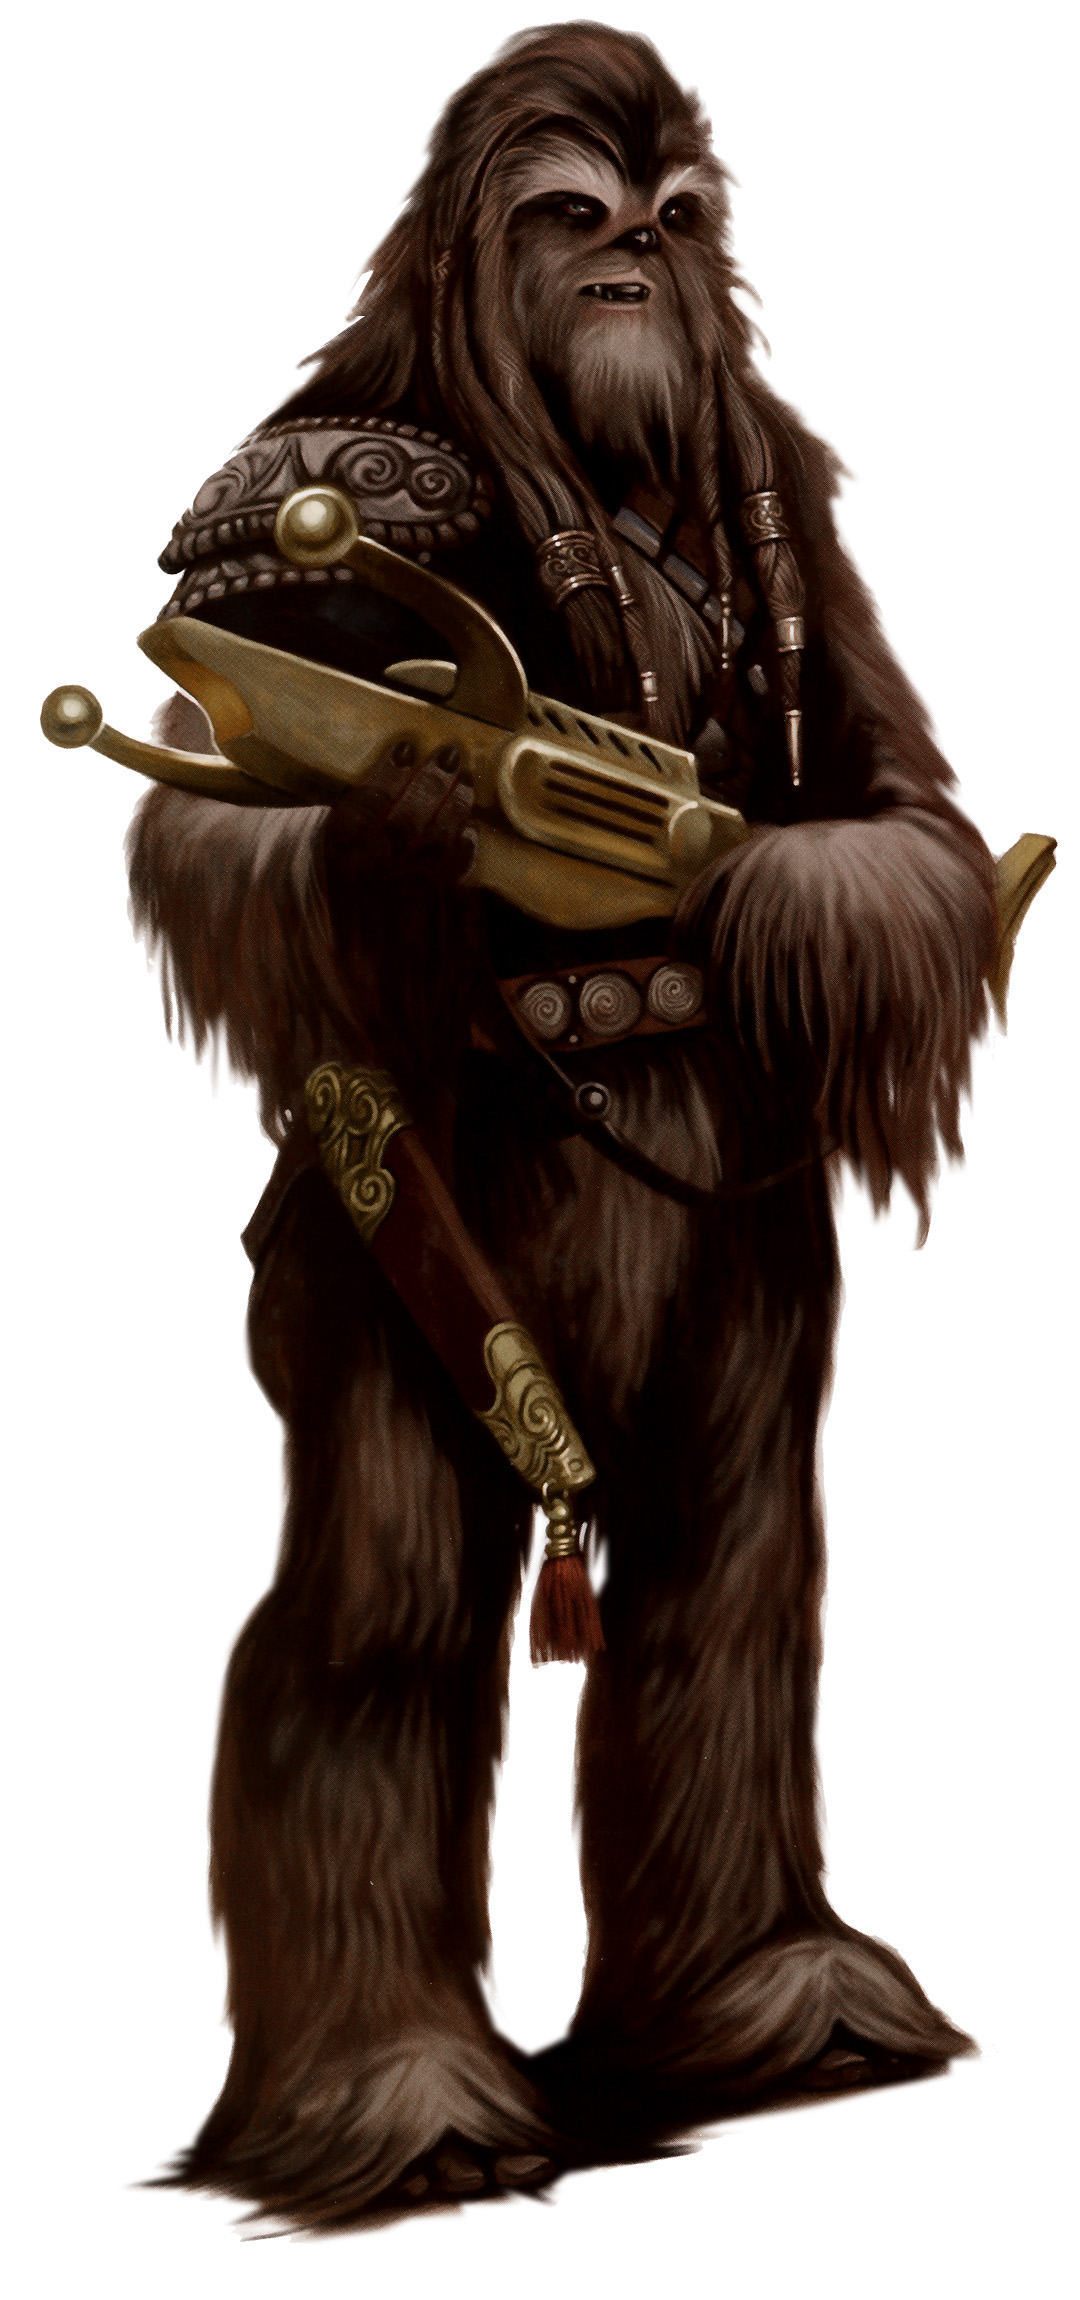
\includegraphics[width=1\linewidth]{../img/species/wookie}
\end{minipage}%
\hfill%
\begin{minipage}{0.7\textwidth}\raggedleft
	\begin{itemize}
		\item \textbf{Seuil de blessure :} 14 + Vigueur 
		\item \textbf{Seuil de stress :} 8 + Volonté 
		\item \textbf{Expérience de départ :} 90 XP
		\item \textbf{Capacité spéciale :} les Wookies commencent le jeu avec 1 rang en \textbf{Pugilat}. Ils ne peuvent cependant pas dépasser le rang 2 dans la compétence choisie à la création de perso.	\textbf{Rage wookie :} quand un Wookie est blessé, ses attaques de \textbf{Pugilat} et de \textbf{Corps à corps} infligent +1 de dégâts. Quand un Wookie subit au moins 1 blessure critique, elles infligent +2 de dégâts.
	\end{itemize}
\end{minipage}
\clearpage

\section{Choisir une carrière (ldr p. 53)}
Choisissez une des 6 carrières qui s'offrent à votre personnage, en respectant au maximum l'histoire que vous avez créée pour lui. Pour chacune de ses carrières Il y a 8 compétences de carrière, mais vous ne pouvez seulement en monter 4 au rang 1 (sauf pour les Droïdes). De plus vous bénéficierez d'une remise quand vous dépenserez de l'expérience dans ces compétences.

\begin{table}[h]
	 \centering
	\begin{tabular}{|m{3.5cm}|m{12cm}|}
		\hline
		\cellcolor{DarkRed} {\large \textcolor{PureWhite}{\textbf{Carrière}}} & \cellcolor{DarkRed} {\large \textcolor{PureWhite}{\textbf{Compétence de carrière}}} \\
		\hline
		Chasseur de prime & Athlétisme, Distance (armes lourdes), Perception, Pilotage (espace), Pugilat, Système D, Vigilance. \\
		\hline
		Colon & Charme, Commandement, Connaissance (culture), Connaissance (éducation), Connaissance (monde du noyau), Négociation, Système D, Tromperie. \\
		\hline
		Explorateur & Astrogation, Calme, Connaissance (bordure extérieure), Connaissance (culture), Connaissance (xénologie), Perception, Pilotage (espace), Survie. \\
		\hline
		Mercenaire & Athlétisme, Corps à corps, Distance (armes légères), Pilotage (planétaire), Pugilat, Résistance, Sang-froid, Vigilance. \\
		\hline
		Contrebandier & Connaissance (pègre), Coordination, Magouilles, Perception, Pilotage (espace), Système D, Tromperie, Vigilance. \\
		\hline
		Technicien & Astrogation, Connaissance (Bordure extérieure), Coordination, Informatique, Mécanique, Perception, Pilotage (planétaire), Sang-froid. \\
		\hline
	\end{tabular}
\end{table}
\clearpage

\section{Choisir une spécialité (ldr p. 53)}
Choisissez une des 3 spécialités par carrière qui s'offrent à votre personnage, en respectant au maximum l'histoire que vous avez créé pour lui. Pour chacune de ses carrières Il y a 4 compétences de carrière supplémentaires, mais vous ne pouvez seulement en monter 2 au rang 1 (sauf pour les Droïdes). De plus vous bénéficierez d'une remise quand vous dépenserez de l'expérience dans ces compétences.

\begin{center}
	\begin{tabular}{|m{3cm}|m{3cm}|p{10cm}|}
		\hline
		\cellcolor{DarkRed} {\large \textcolor{PureWhite}{\textbf{Carrière}}} & \cellcolor{DarkRed} {\large \textcolor{PureWhite}{\textbf{Spécialité}}} & \cellcolor{DarkRed} {\large \textcolor{PureWhite}{\textbf{Compétences de carrière bonus}}} \\
		\hline
		Chasseur de prime & Assassin & Corps à corps, Discrétion, Distance (armes lourdes), Magouilles. \\
		\cline{2-3} & Expert en gadgets & Coercition, Distance (armes légères), Mécanique, Pugilat. \\
		\cline{2-3} & Expert en survie & Connaissance (xénologie), Perception, Résistance, Survie. \\ 
		\hline
		Colon & Médecin & Calme, Connaissance (éducation), Médecine, Résistance. \\
		\cline{2-3} & Diplomate & Charme, Coercition, Connaissance (mondes du noyau), Tromperie. \\
		\cline{2-3} & Erudit & Connaissance (bordure extérieure), Connaissance (pègre), Connaissance (xénologie), Perception. \\
		\hline
		Explorateur & Bourlingueur & Astrogation, Coordination, Négociation, Système D. \\
		\cline{2-3} & Eclaireur & Athlétisme, Médecine, Pilotage (planétaire), Survie. \\
		\cline{2-3} & Négociant & Connaissance (mondes du noyau), Connaissance (pègre), Négociation, Tromperie. \\
		\hline
		Mercenaire & Garde du corps & Artillerie, Distance (armes lourdes), Perception, Pilotage (planétaire). \\
		\cline{2-3} & Maraudeur & Coercition, Corps à corps, Résistance, Survie. \\
		\cline{2-3} & Soldat à louer & Artillerie, Commandement, Distance (armes lourdes), Sang-froid. \\
		\hline
		Contrebandier & Pilote & Artillerie, Astrogation, Pilotage (espace), Pilotage (planétaire). \\
		\cline{2-3} & Vaurien & Calme, Charme, Distance (armes légères), Tromperie. \\
		\cline{2-3} & Voleur & Informatique, Discrétion, Magouilles, Vigilance. \\
		\hline
		Technicien & Mécanicien & Magouille, Mécanique, Pilotage (espace), Pugilat. \\
		\cline{2-3} & Tech Hors-la-loi & Connaissance (éducation), Connaissance (pègre), Mécanique, Système D. \\
		\cline{2-3} & Slicer & Connaissance (éducation), Connaissance (pègre), Informatique, Discrétion. \\
		\hline
	\end{tabular}
\end{center}

\section{Investir les points d'expérience (ldr p. 92)}
Il est temps maintenant de distribuer vos points d'expérience. Vous pouvez avec ces points, augmenter une caractéristique ou le rang d'une compétence, acheter un talent d'une spécialité voir même acheter une nouvelle spécialité.

\begin{center}
	\begin{tabular}{|p{4cm}|p{6cm}|p{6cm}|}
		\hline
		\cellcolor{DarkRed} {\large \textcolor{PureWhite}{\textbf{Options}}} & \cellcolor{DarkRed} {\large \textcolor{PureWhite}{\textbf{Coût}}} & \cellcolor{DarkRed} {\large \textcolor{PureWhite}{\textbf{Limites lors de la création de personnages}}} \\
		\hline
		Augmentation de caractéristiques & 10 fois le rang de caractéristique acheté, chaque rang doit être acheté séparément. & Une caractéristique est limitée à 5 à la création de personnage et ne peut être augmentée qu'à la création \\
		\hline
		Augmentation de compétences & 5 fois le rang de caractéristique acheté, chaque rang doit être acheté séparément. (+5 xp pour des compétences hors carrière) & Une compétence est limitée à 2 à la création de personnage \\
		\hline
		Achat de talents de spécialités & Dépend de la place du talent en question sur l'arborescence & Limites habituelles \\
		\hline
		Achat de nouvelles spécialités & 10 fois le nombre de spécialités une fois que la nouvelle sera acquise (+10 xp pour les spécialités hors carrière) & Limites habituelles \\
		\hline		
	\end{tabular}
\end{center}

\section{Déterminer les attributs dérivés (ldr p. 94)}

\begin{itemize}
	\item Le seuil de blessure se calcule comme indiqué lors de la sélection de l'espèce.
	\item Le seuil de stress se calcule comme indiqué lors de la sélection de l'espèce.
	\item La Défense est par défaut de 0, elle augmente grâce à l'équipement et les talents.
	\item La valeur d'encaissement est égale à votre \textbf{Vigueur}. 
\end{itemize}

\section{Déterminer les motivations (ldr p. 94)}
Lors de la création du personnage, un joueur peut lancer un D10 sur la table ci-dessous pour déterminer sa motivation principale ou la créer de toutes pièces (avec l'accord du MJ).

\begin{table}[h]
	\centering
	\begin{tabular}{|p{1cm}|p{7cm}|}
		\hline
		\centering{\cellcolor{DarkRed} {\large \textcolor{PureWhite}{\textbf{D10}}}} & \cellcolor{DarkRed} {\large \textcolor{PureWhite}{\textbf{Motivation}}} \\
		\hline
		\centering{1 -- 3} & Ambition \\
		\hline
		\centering{4 -- 6} & Cause \\
		\hline
		\centering{7 -- 9} & Relations \\
		\hline
		\centering{10} & Lancez une fois dans deux catégories au choix \\
		\hline	
	\end{tabular}
\end{table}

Puis lancez un D100, ou choisissez sur accord du MJ, pour déterminer la motivation spécifique dans le tableau correspondant à la motivation générale pré sélectionnée.

\subsection*{Ambitions spécifiques}
\begin{table}[h]
	\centering
	\begin{tabular}{|m{2cm}|m{13cm}|}
		\hline
		\centering{\cellcolor{DarkRed} {\large \textcolor{PureWhite}{\textbf{D100}}}} & \cellcolor{DarkRed} {\large \textcolor{PureWhite}{\textbf{Résultat}}} \\
		\hline
		\centering{01 -- 10} & \textbf{Amitié :} le personnage cherche à être apprécié et déploie des trésors d'imagination pour faire bonne impression. Il peut ou non avoir l'instinct grégaire, et compte sur ses actes et exploits pour se faire des amis. \\
		\hline
		\centering{11 -- 20} & \textbf{Amour :} le personnage est animé par l'amour ou l'intimité. Il a déjà une âme sœur ou s'efforce de trouver celle qui lui est destinée. \\
		\hline
		\centering{21 -- 30} & \textbf{Liberté :} le personnage souhaite être libre de faire ce qu'il veut. Il peut s'agir d'u désir irrépressible de surmonter une des ses Obligations ou de voir d'autres individus se défaire des fers de la servitude sous toutes ses formes. \\
		\hline
		\centering{31 -- 40} & \textbf{Renommée :} le personnage cherche à être propulsé sous les projecteurs et veut devenir célèbre. Il souhaite que ses exploits soient diffusés sur le HoloNet et se délecte des attentions de ses fans et partisans. \\
		\hline
		\centering{41 -- 50} & \textbf{Cupidité :} l'argent est le principal motivateur de ce personnage. Il peut se lancer dans les affaires, investir ou tout simplement se tourner vers le vol. \\
		\hline
		\centering{51 -- 60} & \textbf{Statut :} le personnage souhaite gravir les échelons sociaux, accumuler titres, éloges et félicitations. Il peut être d'origine modeste ou chercher à s'élever encore malgré des conditions de vie déjà très favorable. \\
		\hline
		\centering{61 -- 70} & \textbf{Expertise :} le personnage souhaite exceller dans sa carrière et s'entraine constamment pour atteindre la perfection. \\
		\hline
		\centering{71 -- 80} & \textbf{Soif de voyages/de nouveautés :} le personnage désire ardemment explorer la galaxie et reste rarement très longtemps au même endroit. Il est bien décidé à découvrir des régions reculées et inexplorées, et à contempler tout ce qui mérite de l'être. De même, il peut emprunter la voie de sensations et activités nouvelles, voire de l'hédonisme pur et dur. \\
		\hline
		\centering{81 -- 90} & \textbf{Pouvoir :} le personnage a soif de pouvoir et d'autorité. Ce 'n'est pas forcément un despote dans l'âme, mais il veut contrôler sa situation et ceux qui l'entourent, en améliorant son sort au passage. \\
		\hline
		\centering{91 -- 00} & \textbf{Religion/spiritualité :} le personnage est attiré par une voie religieuse ou spirituelle. Il peut s'agir de préceptes Jedi ou Sith, ou de toute autre croyance. \\
		\hline
	\end{tabular}
\end{table}


	
\subsection*{Causes spécifiques}
\begin{table}[h]
	\centering
	\begin{tabular}{|m{2cm}|m{13cm}|}
		\hline
		\centering{\cellcolor{DarkRed} {\large \textcolor{PureWhite}{\textbf{D100}}}} & \cellcolor{DarkRed} {\large \textcolor{PureWhite}{\textbf{Résultat}}} \\
		\hline
		\centering{01 -- 10} & \textbf{Religion/spiritualité :} le personnage soutient activement une organisation ou croyance religieuse ou spirituelle. Il peut s'agir de préceptes Jedi ou Sith, ou de toute autre croyance. \\
		\hline
		\centering{11 -- 20} & \textbf{Les faibles/la charité :} le personnage se bat pour les opprimés, et n'aime ni les brutes, ni el totalitarisme. Il fait passer les intérêts des nécessiteux avant les siens et n'hésite pas à donner du temps ou de l'argent pour les moins fortunés. \\
		\hline
		\centering{21 -- 30} & \textbf{Droits des non-humains :} le personnage milite pour les droits des non-humains malgré le règne xénophobe de l'Empire. \\
		\hline
		\centering{31 -- 40} & \textbf{Politique locale :} le personnage soutien une cause politique, généralement limitée à une planète ou à un système. Il s'implique activement dans les campagnes de ses candidats et peut même se battre pour le compte d'une organisation politique. \\
		\hline
		\centering{41 -- 50} & \textbf{Reverser l'Empire :} le personnage déteste l'Empire et tout ce qu'il incarne. Il ne compte pas forcément parmi les membres actifs de le Rébellion, mais en soutient les objectifs et apporte son aide à tous ceux qui luttent contre la tyrannie impériale. \\
		\hline
		\centering{51 -- 60} & \textbf{Crime :} le personnage n'a rien contre le marché noir, les mercenaires et autres groupes évoluant en marge de la loi, bien au contraire. Ce n'est pas forcément un criminel, mais il lui arrive d'accorder son aide à des gens douteux, surtout s'il s'agit de proches, d'amis d'enfance, ou si la corruption est profondément ancrée dans sa culture d'origine. \\
		\hline
		\centering{61 -- 70} & \textbf{Emancipation :} le personnage voit l'esclavage et la servitude forcée comme des abominations qu'il faut éradiquer. Il fera tout ce qui est en son pouvoir pour aider ou tenter de libérer les victimes d'esclavage. \\
		\hline
		\centering{71 -- 80} & \textbf{Droits des Droïdes :} le personnage croit dur comme fer que les Droïdes devraient être des membres de plein droit de la société galactique, et non de simples outils ou serviteurs. \\
		\hline
		\centering{81 -- 90} & \textbf{Capitalisme :} le personnage est un capitaliste convaincu et milite pour les droits des marchands, des organisations de commerce et des entreprises, en allant parfois à l'encontre des souhaits de l'Empire et de certains groupe criminels. \\
		\hline
		\centering{91 -- 00} & \textbf{Soutenir l'Empire :} le personnage soutient les buts et méthodes de l'Empire, et fait de son mieux pour que sa cause progresse. Il défendra l'Empire à la première conversation venue et pourra même prendre les armes pour le défendre. \\
		\hline
	\end{tabular}
\end{table}


\subsection*{Relations spécifiques}
\begin{table}[h]
	\centering
	\begin{tabular}{|m{2cm}|m{13cm}|}
		\hline
		\centering{\cellcolor{DarkRed} {\large \textcolor{PureWhite}{\textbf{D100}}}} & \cellcolor{DarkRed} {\large \textcolor{PureWhite}{\textbf{Résultat}}} \\
		\hline
		\centering{01 - 10} & \textbf{Lieu d'origine :} le personnage est très fier de l'endroit où il a grandi. Il peut s'agir d'une planète, d'une ville, d'une station spatiale ou d'un vaisseau. Il s'efforce d'améliorer les conditions de vie des gens qui y habitent et se montre prêt à se sacrifier pour les défendre. \\
		\hline
		\centering{11 - 20} & \textbf{Animal de compagnie :} le personnage est proche d'un animal de compagnie de petite taille qui ne combat pas. \\
		\hline
		\centering{21 - 30} & \textbf{Ami d'enfance :} le personnage entretien des liens avec un ami d'enfance. Même si la galaxie les sépare, il ne souhaite que son bien. \\
		\hline
		\centering{31 - 40} & \textbf{Camarades :} le personnage est loyal envers ceux aux côtés desquels il sert. Il peut s'agir de son groupe de PJ, d'anciens compagnons d'armes ou de partenaires commerciaux. \\
		\hline
		\centering{41 - 50} & \textbf{Frères et sœurs :} le personnage a un ou plusieurs frères et sœurs avec qui il entretient des liens étroits. Il ne s'agit ans doute pas de combattants et cette Motivation peut s'aligner sur une Obligation de famille. \\
		\hline
		\centering{51 - 60} & \textbf{Mentor :} le personnage est très proche d'un mentor, professeur, enseignant ou tout autre individu lui ayant jadis prodigué son soutien, ses connaissances ou sa sagesse. \\
		\hline
		\centering{61 - 70} & \textbf{Parents :} le personnage entretien des liens étroits avec un de ses parents ou les deux, et cherche constamment leur approbation. Il ne s'agit pas forcément d'une situation saine ou fondée sur la solidarité. \\
		\hline
		\centering{71 - 80} & \textbf{Faille/clan étendu :} le personnage a une très grande famille (à moins qu'il ne s'agisse d'un clan ou d'une tribu) qu'il aime profondément. Aussi nombreux soient ces parents, qui cherchent peut-être tous à le gagner à leur cause personnelle, il s'efforce d'obtenir leur approbation et leur réconfort communs. \\
		\hline
		\centering{81 - 90} & \textbf{Compagnon Droïde :} le personnage apprécie tout particulièrement un certain Droïde. Il peut s'agir d'un ancien serviteur familial, de l'astromech de son vaisseau ou de son unité de protocole de confiance. Cela peut aussi être un Droïde PJ. \\
		\hline
		\centering{91 - 00} & \textbf{Vieil ennemi :} le personnage a noué un lien étroit avec un vieil ennemi ou un ancien rival. Bien que les choses soient réglées entre eux, la compétition est peut-être encore très vive. \\
		\hline
	\end{tabular}
\end{table}

\section{Equipement et apparence (ldr p. 97)}
Avant que le jeu ne débute, les PJ reçoivent 500 crédits pour acheter de l'équipement de départ. Ce budget peut être augmenté si le PJ a choisi d'augmenter son Obligation de départ (ldr p. 40). Les joueurs peuvent dépenser cet argent pour s'offrir des objets du Chapitre V du livre de règles (p. 147). Les PJ notent les crédits qu'ils n'ont pas dépensés sur leur feuille et y ajoute 1D100 crédit comme argent de poche pour débuter la partie. Ensuite, les PJ remplissent la section description physique en respectant les limitations de leur espèce (taille, poids, \ldots).

\section{Choisir un vaisseau (ldr p99)}
Le groupe de PJ se réunit pour choisir un vaisseau suivant leur affinité avec l'aventure qu'ils joueront :

\subsection*{Cargo moyen Wayfarer}

\noindent\begin{minipage}{0.3\textwidth}
	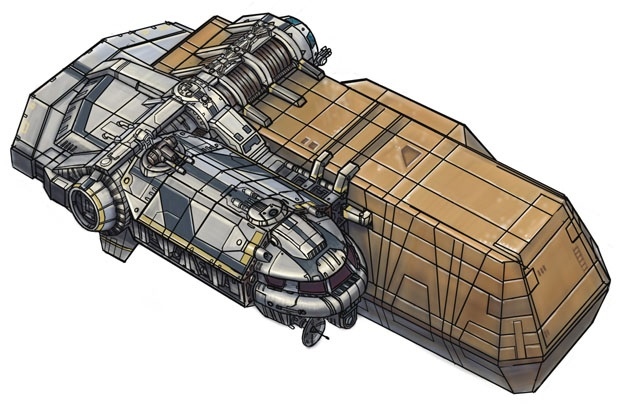
\includegraphics[width=1\linewidth]{../img/species/wayfarer}
\end{minipage}%
\hfill%
\begin{minipage}{0.7\textwidth}\raggedleft
	\begin{itemize}
		\item \textbf{Constructeur :} Chantiers navals de Kuat
		\item \textbf{Hyperdrive :} Primaire (classe 2), secondaire (classe 14)
		\item \textbf{Naviordinateur :} oui
		\item \textbf{Portée des senseurs :} moyenne
		\item \textbf{Equipage :} 1pilote, 1 copilote, 1 ingénieur, 1 responsable de fret, 6 matelots
		\item \textbf{Charge utile :} 850
		\item \textbf{Passagers :} 6
		\item \textbf{Provisions :} 3 mois
		\item \textbf{Emplacements disponibles :} 5
		\item \textbf{Armes :} Quad-laser dorsal (portée proche / arc de tir : dorsal / dégâts 5 / critique 3 / jumelé 3 / précis)
	\end{itemize}
\end{minipage}

\subsection*{Cargo léger YT-1300}

\noindent\begin{minipage}{0.3\textwidth}
	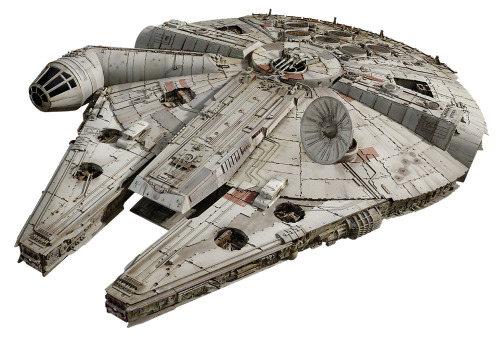
\includegraphics[width=1\linewidth]{../img/species/yt}
\end{minipage}%
\hfill%
\begin{minipage}{0.7\textwidth}\raggedleft
	\begin{itemize}
		\item \textbf{Constructeur :} Corporation Technique Corellienne
		\item \textbf{Hyperdrive :} Primaire (classe 2), secondaire (classe 12)
		\item \textbf{Naviordinateur :} oui
		\item \textbf{Portée des senseurs :} courte
		\item \textbf{Equipage :} 1pilote, 1 copilote/ingénieur
		\item \textbf{Charge utile :} 165
		\item \textbf{Passagers :} 6
		\item \textbf{Provisions :} 2 mois
		\item \textbf{Emplacements disponibles :} 6
		\item \textbf{Armes :} Canon laser monté sur tourelle dorsale et ventrale (portée proche / arc de tir [ventral ou dorsal] : tous / dégâts 6 / critique 3)
	\end{itemize}
\end{minipage}

\subsection*{Vaisseau de Patrouille Firespray}

\noindent\begin{minipage}{0.3\textwidth}
	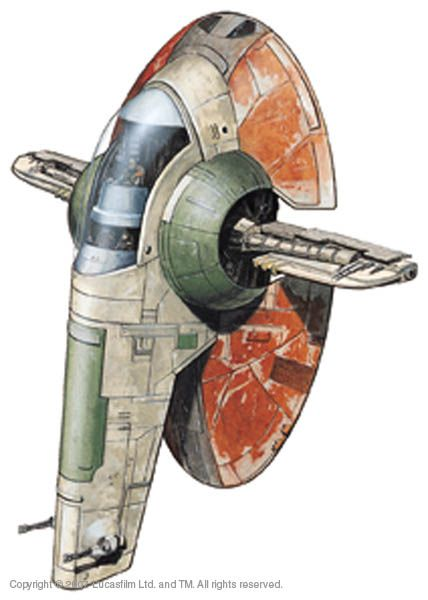
\includegraphics[width=1\linewidth]{../img/species/firespray}
\end{minipage}%
\hfill%
\begin{minipage}{0.7\textwidth}\raggedleft
	\begin{itemize}
		\item \textbf{Constructeur :} Kuat Systems Engineering
		\item \textbf{Hyperdrive :} Primaire (classe 3), secondaire (classe 15)
		\item \textbf{Naviordinateur :} oui
		\item \textbf{Portée des senseurs :} courte
		\item \textbf{Equipage :} 1pilote, 2 gardes
		\item \textbf{Charge utile :} 40
		\item \textbf{Passagers :} 6 (prisonniers)
		\item \textbf{Provisions :} 1 mois 
		\item \textbf{Emplacements disponibles :} 4
		\item \textbf{Armes :} Autoblasters montés à l'avant (portée proche / arc de tir : avant / dégâts 3 / critique 5 / automatique) Rayon tracteur léger monté à l'avant (portée proche / arc de tir : avant / dégâts - / critique - / tracteur 2)
	\end{itemize}
\end{minipage}



\end{document}
